%!TEX root = ../../main.tex


\begin{figure}[!htb]
\centering
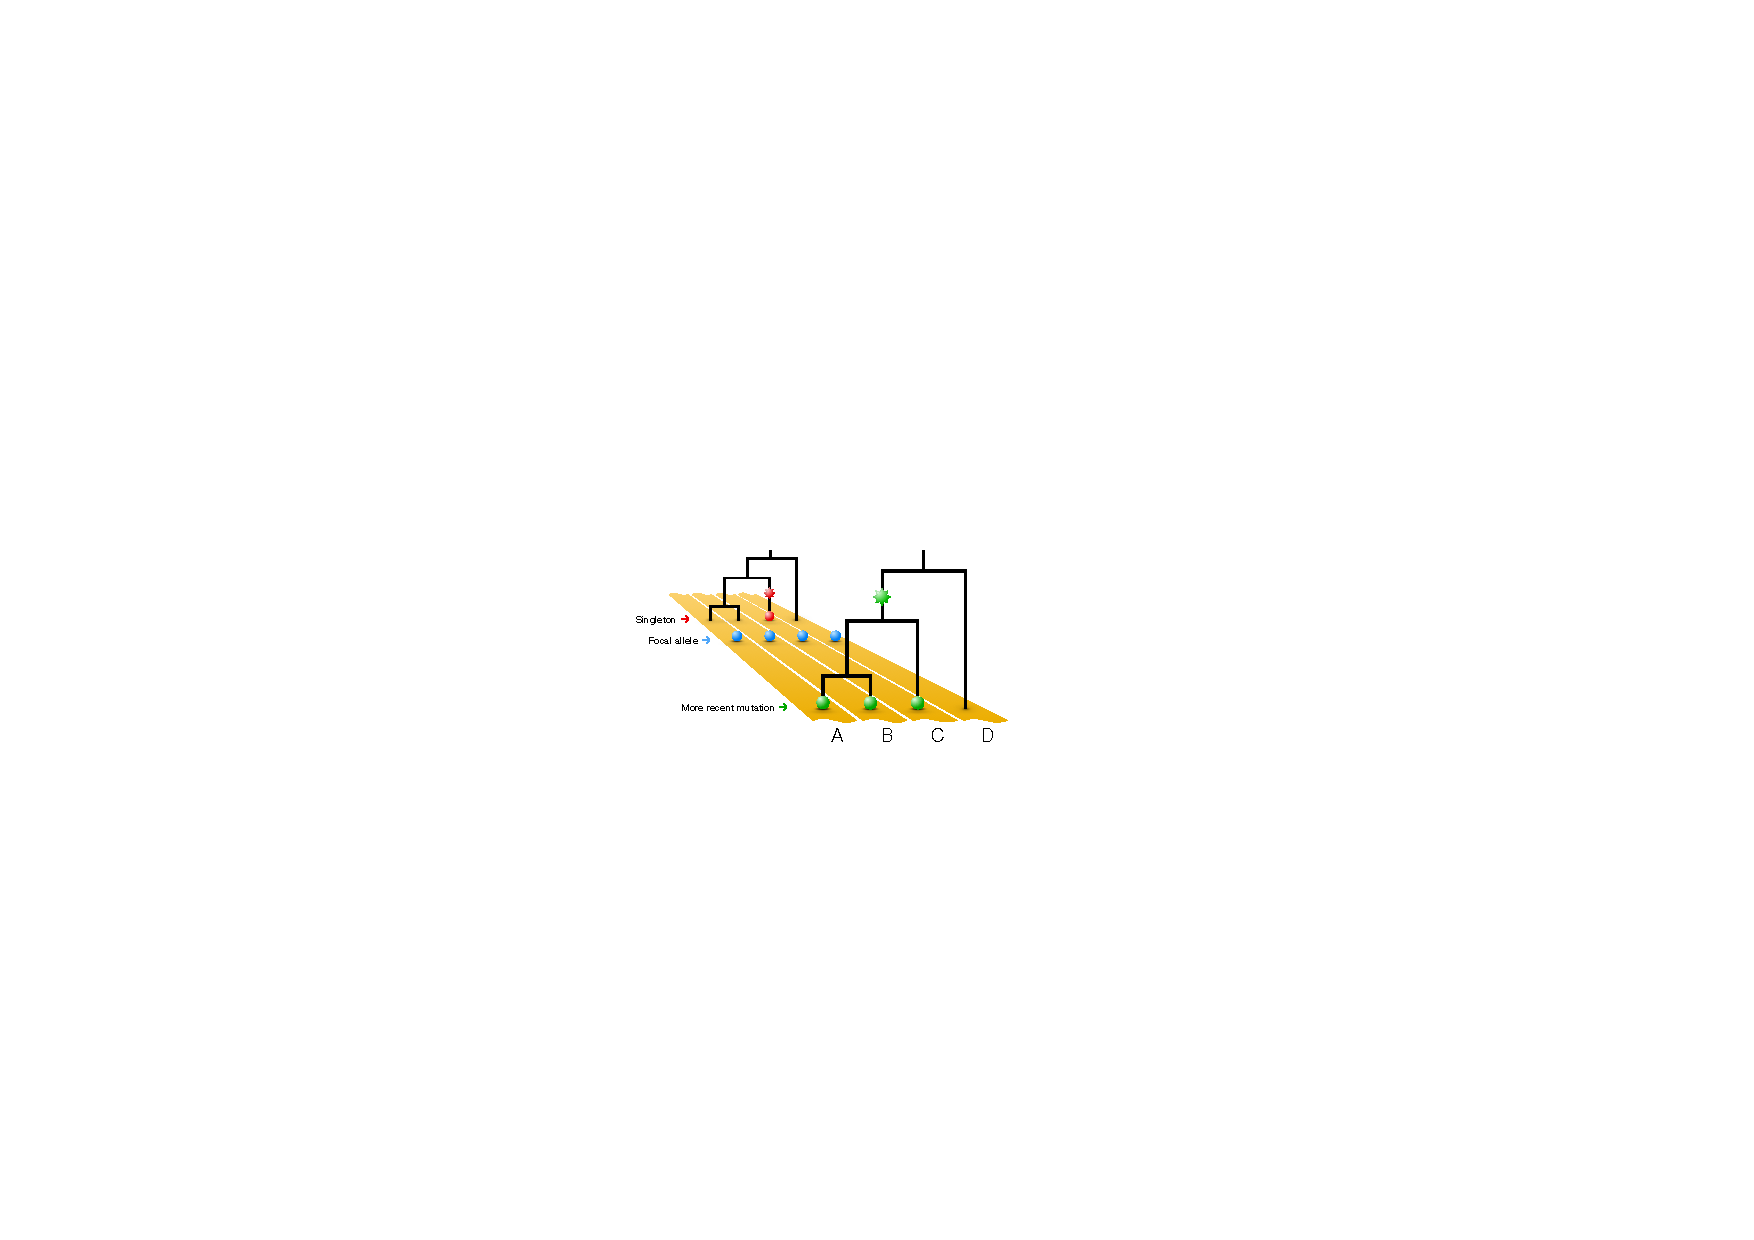
\includegraphics[width=0.9\textwidth]{./img/ch3/info_phase_incons}
\Caption{Illustration of genealogical shared haplotype inconsistency}
{A sample of \n{4} haplotypes is shown which correspond to the haplotype regions that are identicial by descent in \n{4} individuals; \emph{A}, \emph{B}, \emph{C}, and \emph{D}.
The shared haplotype is identified by a focal allele~(\emph{blue}).
Note that there is only \n{1} genealogical tree connecting the \n{4} haplotypes over the region shown; as such, the \n{2} shown trees have the same topology and branch lengths.
In this example, each tree marks the chromosomal position of a genetic variant (not shown for the focal variant), where alleles~(\emph{balls}) derive from mutations~(\emph{stars}) as indicated on each tree.
On the left-hand side, the tree shows a private mutation (singleton) which leads to the observation of the derived allele (\emph{red}) on the shared haplotype in individual \emph{C}.
The tree on the right-hand side shows a mutation that occurred more recently than the mutation that gave rise to the focal allele.
Because it is more recent, the derived allele (\emph{green}) can only be observed in haplotypes in a subtree; \ie the shared haplotypees in individuals \emph{A}, \emph{B}, and \emph{C} in this example.}
{fig:info_phase_incons}
% \vspace{-5pt}
% \hrulefill%
\end{figure}
